% Created 2018-03-12 Mon 16:16
% Intended LaTeX compiler: pdflatex
\documentclass[11pt]{article}
\usepackage[utf8]{inputenc}
\usepackage[T1]{fontenc}
\usepackage{graphicx}
\usepackage{grffile}
\usepackage{longtable}
\usepackage{wrapfig}
\usepackage{rotating}
\usepackage[normalem]{ulem}
\usepackage{amsmath}
\usepackage{textcomp}
\usepackage{amssymb}
\usepackage{capt-of}
\usepackage{hyperref}
\author{Mark Dawson}
\date{\today}
\title{}
\hypersetup{
 pdfauthor={Mark Dawson},
 pdftitle={},
 pdfkeywords={},
 pdfsubject={},
 pdfcreator={Emacs 25.3.1 (Org mode 9.1.6)}, 
 pdflang={English}}
\begin{document}

\tableofcontents

\section{Gitlab Usage}
\label{sec:org4a0911c}
The following document describes steps necessary to use the \href{https://sa2c-gitlab.swansea.ac.uk/}{SA2C GitLab} to manage code on SCW infrastructure.

\subsection{Setting up Git}
\label{sec:org3a2d41f}
Git can be used from the login nodes (e.g. ssl001) to pull code from the
outside. Note however that in order to do this, a proxy connection should be
used. Please ensure that you are running version 2.9.5 of git.

Note: If you have previously installed git, and are using git 1.9.0, you will
   need to remove any references that you have added to your profile files (.bashrc, .profile etc). 

In order to have git available, log into a job submission node (e.g. ssl001) and
   open the .bashrc file. You can do this on the command line by typing:

\begin{verbatim}
nano ~/.bashrc
\end{verbatim}

At the end of the file, add the following lines:

\begin{verbatim}
module load git/2.9.5
export https_proxy=https://10.211.143.6:8080
\end{verbatim}

You will need to log out of the job submission node and back in again in order
for these changes to take effect. You may now test your git setup. You can do
this easily by listing the branches of a remote repository, for example SLURM,
using the following command:

\begin{verbatim}
git ls-remote -h https://github.com/SchedMD/slurm
\end{verbatim}

If unsuccessful this command will return an error message, such as:

\begin{verbatim}
fatal: unable to access 'https://github.com/SchedMD/slurm/': Failed to connect to github.com port 443: No route to host
\end{verbatim}

If you see a list of remote heads for the SLURM workload manager, the previous
commands have been successful. Below is a sample output given today, note that
exact output that you see will likely differ.

\begin{verbatim}
59c02e4f984ac9a4eb648166b8744132f7238e63	refs/heads/b4847
2fdf92d782d9920583ccfa2d6ad28b3ebd0b846b	refs/heads/bug_4584
bc22cda6dee857959e6f2107a10b3704c884fd81	refs/heads/cli_filter
d04f3b0712f67667d2de91852863fd84bd7b3228	refs/heads/cray_pack
128be108d49c3389db4f3d0f342d3e09f9465c88	refs/heads/dw_up06
ec8c44e7175c864e994a16e575b7e0d23e692ff4	refs/heads/federation
beda3baa537027ef77cfd43d65817b9735ab1998	refs/heads/fedlab
a2ed2a0e1730edf56a4547ff920dfbdbcb3c7b27	refs/heads/influxdb
94f64c34d75714f6f0baa1d1aec8b1cb50ec5321	refs/heads/loadleveler
9c812ab57bb4d4e79ee7e888420b83c0ce65c1f3	refs/heads/master
b3db0fc049f86a9e71355eb6d6982a228a0b2095	refs/heads/max_priority
451675e755b7c7fdcd322fedf93ab6b2ce0e15a3	refs/heads/scontrol_json
6793b46de9c7a8780a2fe66cb6bc1dfa0fbbe625	refs/heads/shmem_pmi
acd6440b45254ceea87e606d2ca6b5df0cb86116	refs/heads/simulator
[[https://sa2c-gitlab.swansea.ac.uk][https://sa2c-gitlab.swansea.ac.uk]], and click the "Register" link, as shown in
4876672c6b474c23e19c76d666101aa72b4e1562	refs/heads/slurm-1.0
bfc14bf3405c2386ce303fea08b67dd4778e3923	refs/heads/slurm-1.1
93d5dcb63f041b71e309c35a3221a92ee57335e7	refs/heads/slurm-1.2
616fc7b3889fe0c2fb9b74bedbe647a9debd7f5a	refs/heads/slurm-1.3
bda0a436fe734303c0329055c004d4a5758dbc17	refs/heads/slurm-14.03
4109fcbfd71a8c5b0fffd284f35c55155f4fa513	refs/heads/slurm-14.11
b3107d89747875de42e2ca7c14ce1d5dd283c99a	refs/heads/slurm-15.08
da4397efa315745930b15367f2956f79597c5b9d	refs/heads/slurm-16.05
252d0573a6cec490acee501903a3f0af6c5b1a84	refs/heads/slurm-17.02
6d4518feb2578c21fab675f42b639eb02844c17f	refs/heads/slurm-17.11
bbdd07c1d8d667e1a3b387c10951058b2628af73	refs/heads/slurm-2.0
5a6f41e2b91347c6a34ba9c7ee6e6bfe2836454a	refs/heads/slurm-2.1
a0e6bbde1d9d8386aa729b5883f11530902fff08	refs/heads/slurm-2.2
ff26cc50db9e2fe2f9745a16c8c59fd3e0bd7ae8	refs/heads/slurm-2.3
29c2661a4410a0621ddace5881122106f4cb2a11	refs/heads/slurm-2.4
04f06338896c14e83a3d5fb0dec81c60d4aca071	refs/heads/slurm-2.5
63332d41b3232a1c7ceda976992b8ca2a22dcc39	refs/heads/slurm-2.6
594881bb4dbfbcc5868e36e8dc79ffc35d748a58	refs/heads/step_alloc
d856b526c7364b2b9bd0e0a5c15cc84d9e74edc6	refs/heads/tresbilling_test
ff8d659cba6005f41c3cc45356593d5ab093c5fe	refs/heads/usage
f153ac81b8e3c0c6553104bfa73041fc776675f3	refs/heads/xtconsumer
\end{verbatim}


\subsection{Gitlab user registration}
\label{sec:orgd56f655}
In order to access code on our gitlab servers, you will need to create a
user account, if you have done so already you may skip this section. Visit
\href{https://sa2c-gitlab.swansea.ac.uk}{https://sa2c-gitlab.swansea.ac.uk}, and click the "Register" link, as shown in
the image:

\begin{figure}[htbp]
\centering
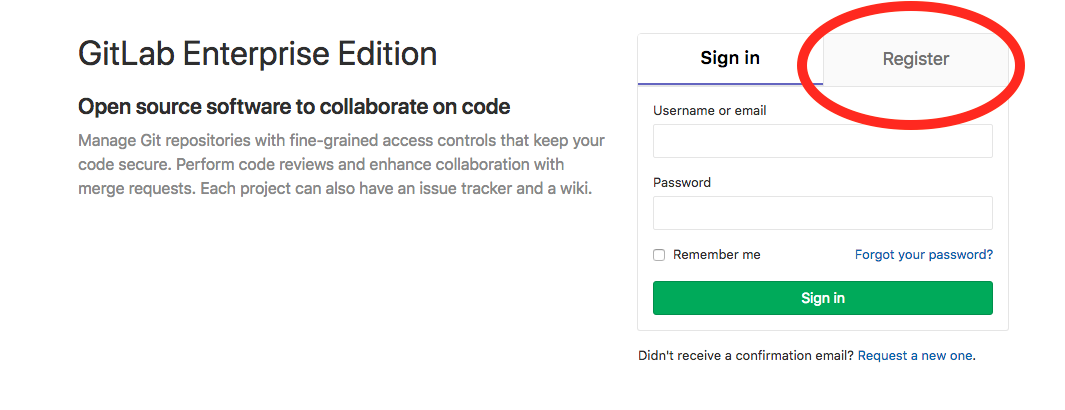
\includegraphics[width=.9\linewidth]{./gitlab_login_page.png}
\caption{GitLab sign in page}
\end{figure}


Complete your details, ensuring that you use your @swansea.ac.uk email address,
and click Register.

\subsection{GitLab project access}
\label{sec:orgc78852f}
On first registration, you will not be able to see the code for any projects.
Each project should have been assigned at least one user with "master" rights, who will in
turn be able to add other users to the repository. The project
owner may know the identity of the "master" user. If the identity is not known,
or no master user has yet been assigned for this project, contact SA2C on
\href{https://sa2c-gitlab.swansea.ac.uk}{https://sa2c-gitlab.swansea.ac.uk}. Note that master users are able to assign
other master users for their repositories.

\subsection{Granting user access (for repository master users)}
\label{sec:orgc785794}
This section contains instructions for users with "master" rights to a repository to
grant repository access to other users. Users who are not a master user may skip
this section.

\begin{itemize}
\item Browse to the project page (Projects -> Your Projects -> click on the project
name).
\item Click "Settings" and then "Members" on the left hand side sidebar
\item Select the user under "Select members to invite"
\item Choose an appropriate role (i.e. permission level) for the user and an
expiration date if necessary. You may click the "Read more" link to learn more
about available permissions.
\item Click "Add to project" to allow the user repository access.
\end{itemize}

\subsection{Downloading the source code (the easy way)}
\label{sec:org0b5e0f8}
Once gitlab access is set up, you can download the source directly from our
gitlab pages. The easiest way is to visit the project page and copy the URL
project MyExampleProject, in the image below, this would be
\url{https://sa2c-gitlab.swansea.ac.uk/test.user/MyExampleProject}.

\begin{figure}[htbp]
\centering
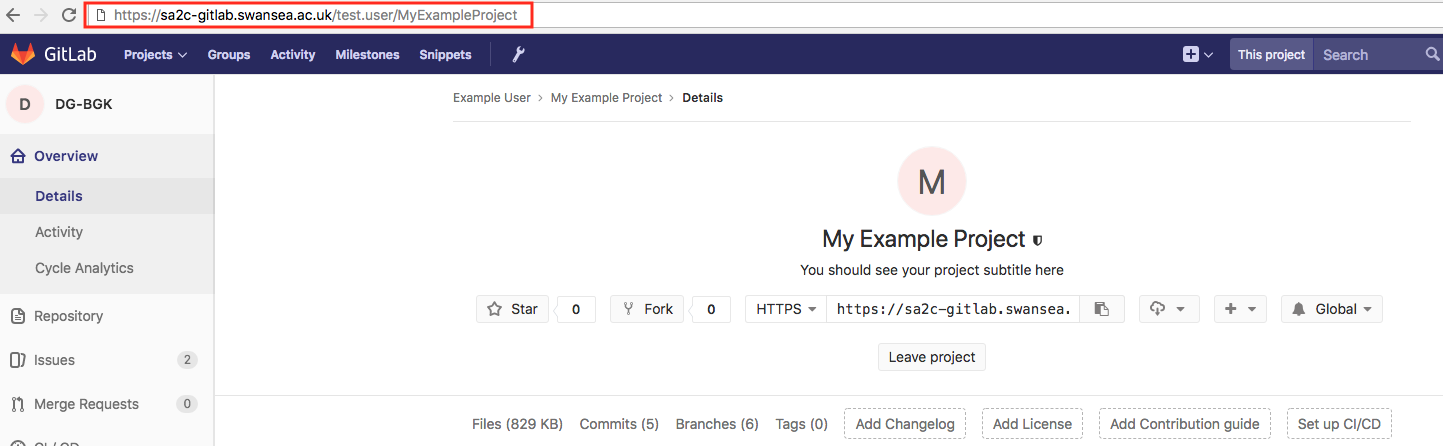
\includegraphics[width=.9\linewidth]{./download_link.png}
\caption{Project page}
\end{figure}

Now, on a job submission node (e.g. ssl001), you can download the source using:

\begin{verbatim}
git clone https://sa2c-gitlab.swansea.ac.uk/test.user/MyExampleProject
\end{verbatim}

You will be prompted for you username, which is the email address with which you
signed up for GitLab, and your password. The source will be downloaded to a
directory in the current working directory.

\subsection{Downloading the source code (the fast way)}
\label{sec:org2074f81}
If you wish to avoid typing your username and password every time, authentication using
ssh keys is also possible. In order to set this up, some additional steps are
required. First, click on "Settings" in the user profile menu in the top right
of your screen, as shown:
\begin{center}
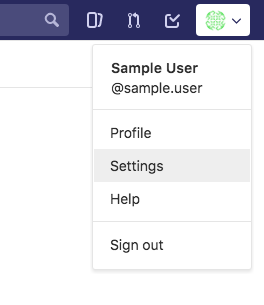
\includegraphics[width=.9\linewidth]{./user_profile.png}
\end{center}
In the left hand sidebar, click "SSH Keys". Now need to grab the contents of
your ssh key, available on the SCW cluster in the file \textasciitilde{}/.ssh/id\(_{\text{rsa.pub}}\). Copy
the contents of the key into the "Key" field and give it a recognisable title.
Click "Add key" to add the key. In order to clone, you will now need to select
the SSH protocol in the protocol field:
\begin{center}
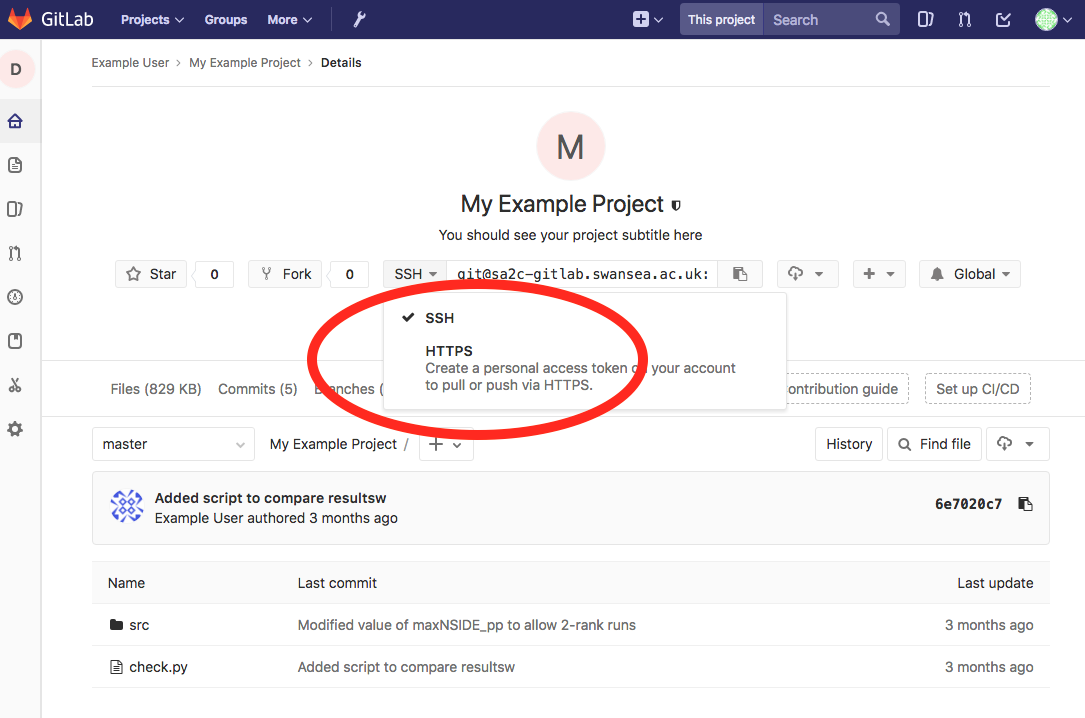
\includegraphics[width=.9\linewidth]{./ssh_protocol.png}
\end{center}
and copy the URL shown next to it. The git command for the previous repository
would look something like:
\begin{verbatim}
git clone git@sa2c-gitlab.swansea.ac.uk:test.user/MyExampleProject.git
\end{verbatim}
Note the git@ at the start of the URL.
\end{document}